\section{Konditionerings apparat}
Konditioneringsapparatet er opbygget af flere blokke, som kan ses på figur \ref{fig:BDD(SystemOverview)}. Blok difinition diagrammer beskriver relationerne mellem blokke, så som sammenhæng, forening og specialisering. I denne sammenhæng beskriver figur \ref{fig:BDD(SystemOverview)} opbygningen af konditioneringsapparatet. 
\begin{figure}[H]
	\centering
	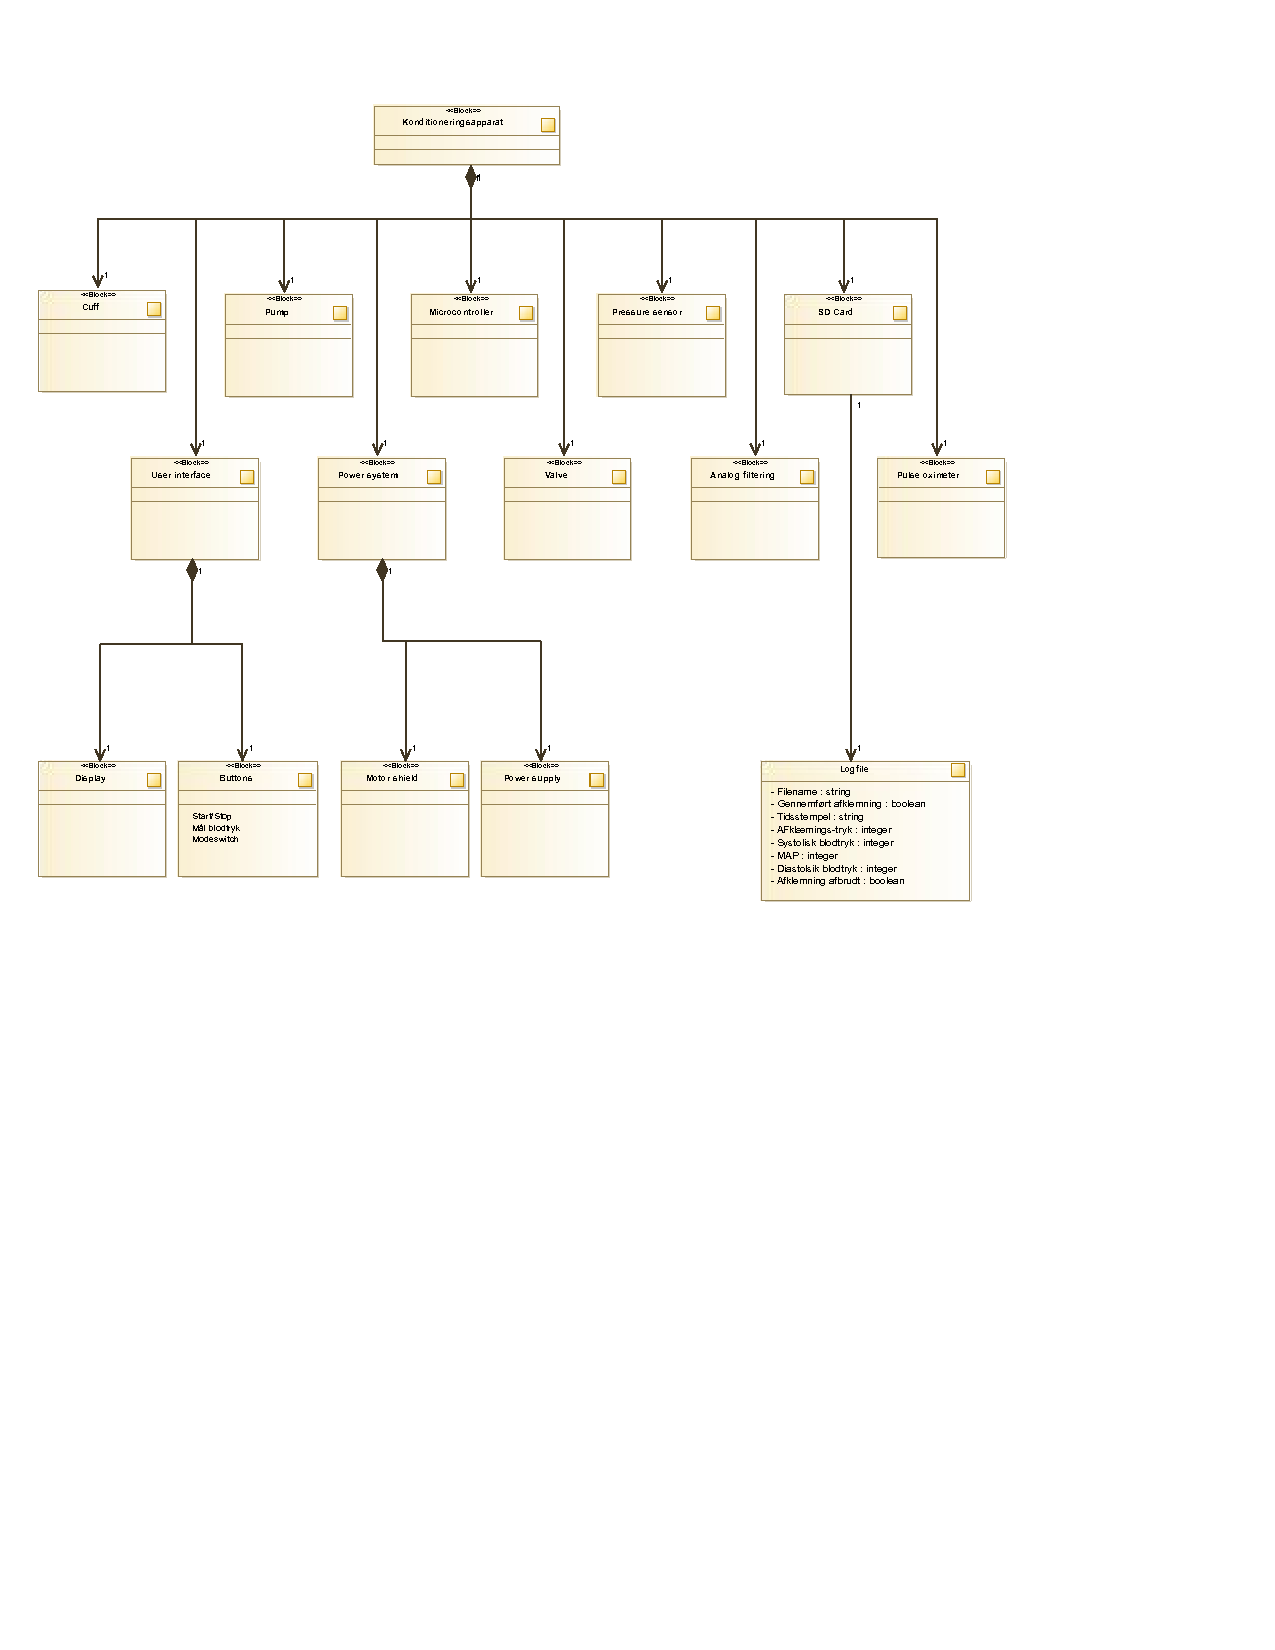
\includegraphics[width=0.9\textwidth]{billeder/BDD(SystemOverview).pdf}
	\caption{Block difinition diagram over konditioneringsapparatet.}\label{fig:BDD(SystemOverview)}
\end{figure}

\subsection{Oscilumetrisk blodtryks apparat}
Den oscillometriske blodtryks måle metode, beskrevet i afsnit \ref{noninvasivBloodpressureMeasurement}, blev implementeret som beskrevet i implementeringsdokumentet\fixme{reff: implementeringsdokument} og resultaterne der af er beskrevet følgende.

Det pulserende signal fra tryksensoren, som blodtryksmåleren analyserer er i sin rå (ubehandlet) tilstand støjfyldt. Signalet beskrevet i afsnit \ref{noninvasivBloodpressureMeasurement} på figur \ref{fig:OscillometriskMetode} er meget rent og amplitude højderne danner en flot parabel kurve. På figur \ref{fig:rawPulseSignal} ser det pulserende signal indhyldet i støj. Kurven er stødt faldende, fordi trykket i manchetten langsomt lukkes ud. Ydermere observeres der også varierende amplitudehøjder, som ikke er stødt stigende/faldende, men virker  tilfældigheder.  

\begin{figure}[H]
	\centering
	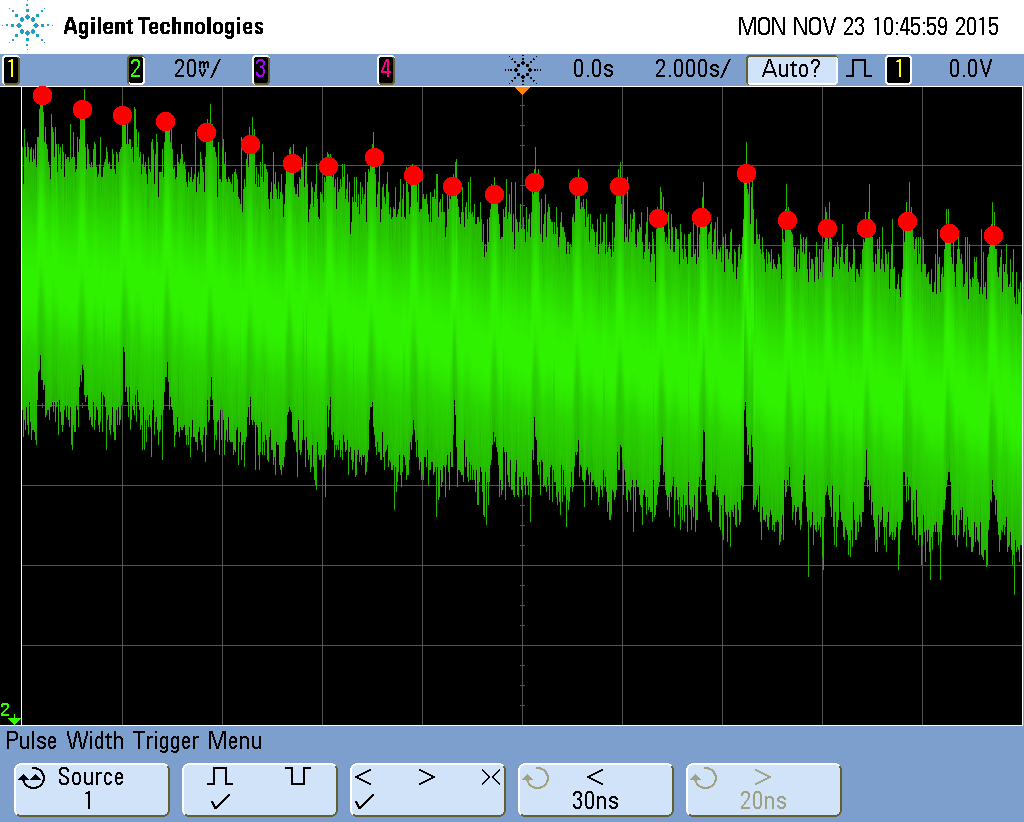
\includegraphics[trim={0 7cm 0 1.5cm},clip, width=1\textwidth]{billeder/rawPulseSignalPeaks.png}
	\caption{Osclilloskops måling af rå signal fra blodtryksmåling, med konditioneringsapparatet. De røde cirkler er pulse oscillotionernes højeste punkt}\label{fig:rawPulseSignal}
\end{figure}

Efter analog filtrering af det rå signal ved en endnu en blodtryksmåling med konditioneringsapparatet, ses at

\begin{figure}[H]
	\centering
	\subbottom[Stigende]{%
		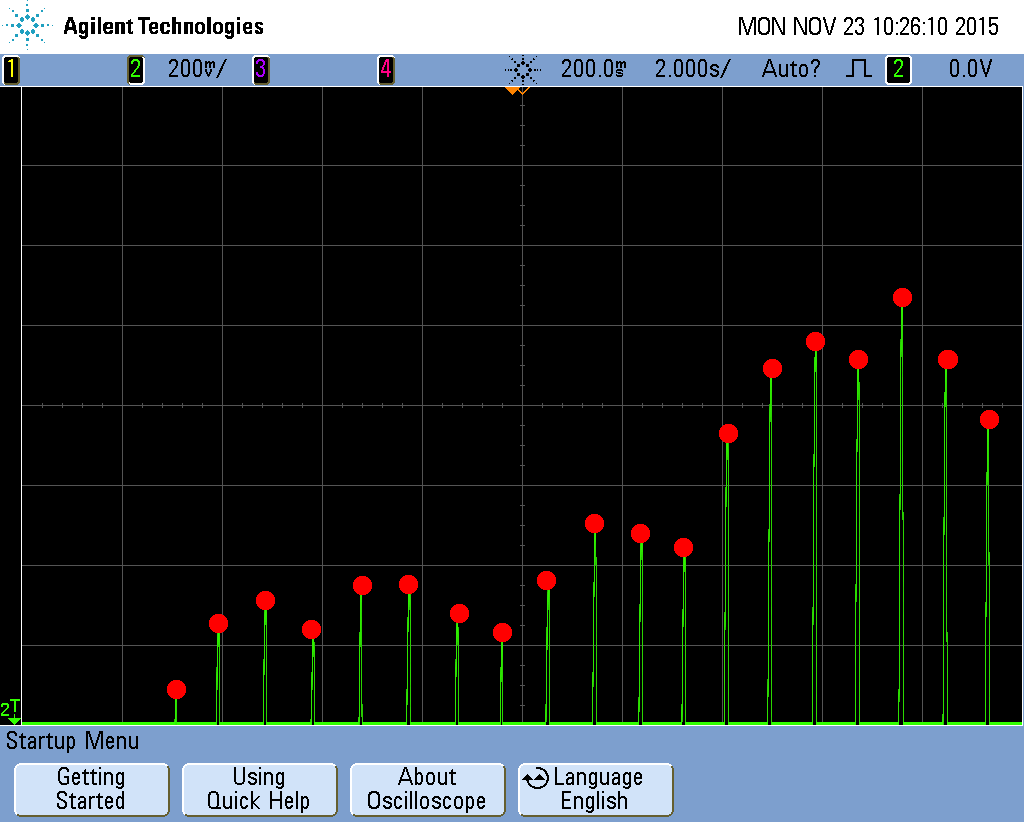
\includegraphics[trim={0 3.3cm 0 1.5cm},clip, width=0.328\textwidth]{billeder/filteredPulseSignalPeaks1.png}}
	\subbottom[Højdepunkt]{%
		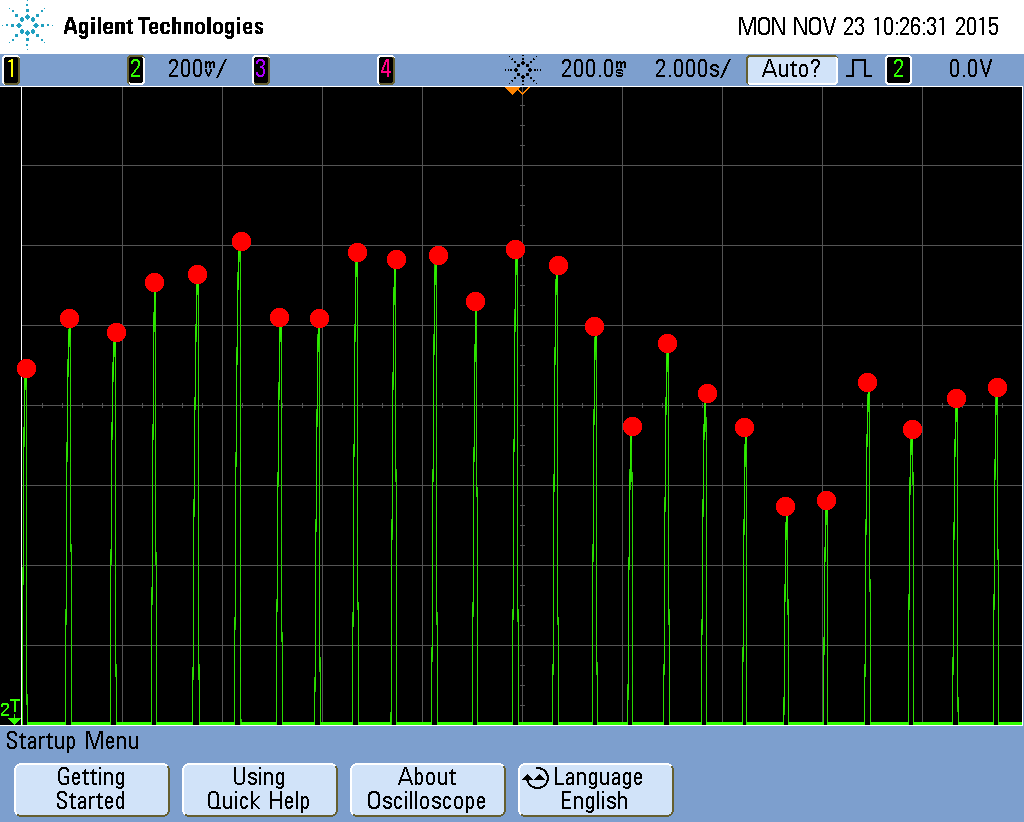
\includegraphics[trim={0 3.3cm 0 1.5cm},clip, width=0.328\textwidth]{billeder/filteredPulseSignalPeaks2.png}}
	\subbottom[Faldende]{%
		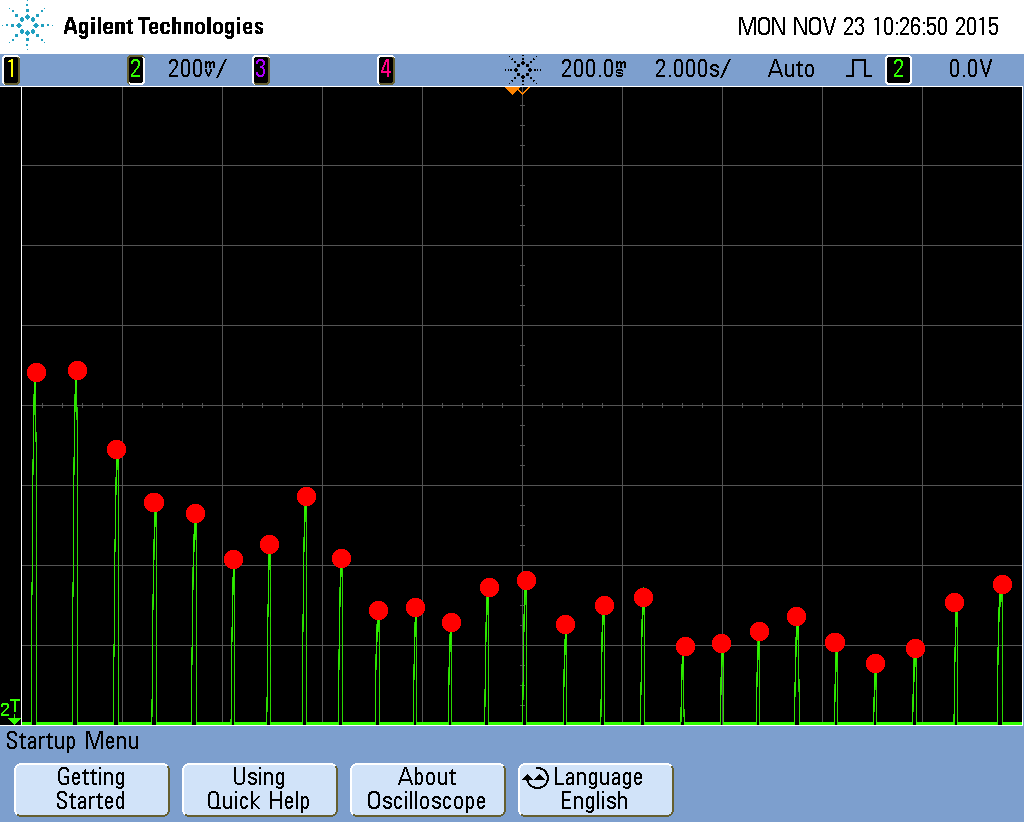
\includegraphics[trim={0 3.3cm 0 1.5cm},clip, width=0.328\textwidth]{billeder/filteredPulseSignalPeaks3.png}}
	\caption{Osclilloskops måling af filtreret signal af blodtryksmåling, med konditioneringsapparatet. (a) er første del af blodtryksmålingen, (b) er abdeb De røde cirkler er pulse oscillotionernes højeste punkt}\label{fig:filteredPulseSignal}
\end{figure}


\subsection{Fikseret-ratio} \label{Fikseret-ratio}